\chapter{Unsupervised Learning: Clustering and PCA}
\label{chap:unsupervised}
\chapterguide
  {You should understand feature scaling, validation, and supervised targets.}
  {distinguish supervised from unsupervised learning; run k-means clustering; interpret cluster limitations; and use PCA to represent correlated numeric features in fewer dimensions.}

\section{Unsupervised learning has no target label during fitting}
Supervised learning asks how features predict a known outcome. Unsupervised learning searches for structure in the feature space itself. Common tasks include clustering, dimensionality reduction, anomaly detection, and representation learning.

\section{K-means searches for compact groups}
K-means chooses \(k\) cluster centres and assigns each observation to the nearest centre, repeating assignment and centre updates to reduce within-cluster squared distance.

\begin{utpfig}[K-means loop]{K-means alternates between assigning observations and recomputing centres until assignments stabilise or improvement becomes negligible.}{fig:kmeans-loop}
\begin{tikzpicture}[x=\linewidth,y=1cm,
  stage/.style={draw=UTPBlue!70,fill=UTPPaleBlue,rounded corners=1.5mm,
    line width=0.6pt,text width=0.26\linewidth,minimum height=1.55cm,
    inner xsep=2.5mm,inner ysep=2mm,align=center,
    font=\scriptsize\color{UTPNavy}},
  flow/.style={-{Stealth[length=2mm,width=1.5mm]},
    line width=0.8pt,draw=UTPTeal},
  repeatflow/.style={flow,draw=UTPMuted,rounded corners=2mm}]
\node[stage] (init) at (0,0) {\textbf{1. Initialise}\\[4pt]
  Choose $k$\\initial centres};
\node[stage] (assign) at (0.335,0) {\textbf{2. Assign}\\[4pt]
  Assign each observation\\to its nearest centre};
\node[stage,draw=UTPTeal!80,fill=UTPPaleTeal] (update) at (0.670,0)
  {\textbf{3. Update}\\[4pt]
   Recompute the\\cluster centres};
\draw[flow] (init.east) -- (assign.west);
\draw[flow] (assign.east) -- (update.west);
\draw[repeatflow] (update.south) -- (0.670,-1.4) --
  node[midway,below=3pt,font=\scriptsize\color{UTPMuted}]
    {Repeat until convergence}
  (0.335,-1.4) -- (assign.south);
\end{tikzpicture}
\end{utpfig}


\begin{utpfig}[K-means clusters in petal space]{The algorithm partitions observations according to distance from learned centres. The labels ``cluster 1'' etc. are arbitrary; only the geometry matters during fitting.}{fig:unsup-kmeans-example}
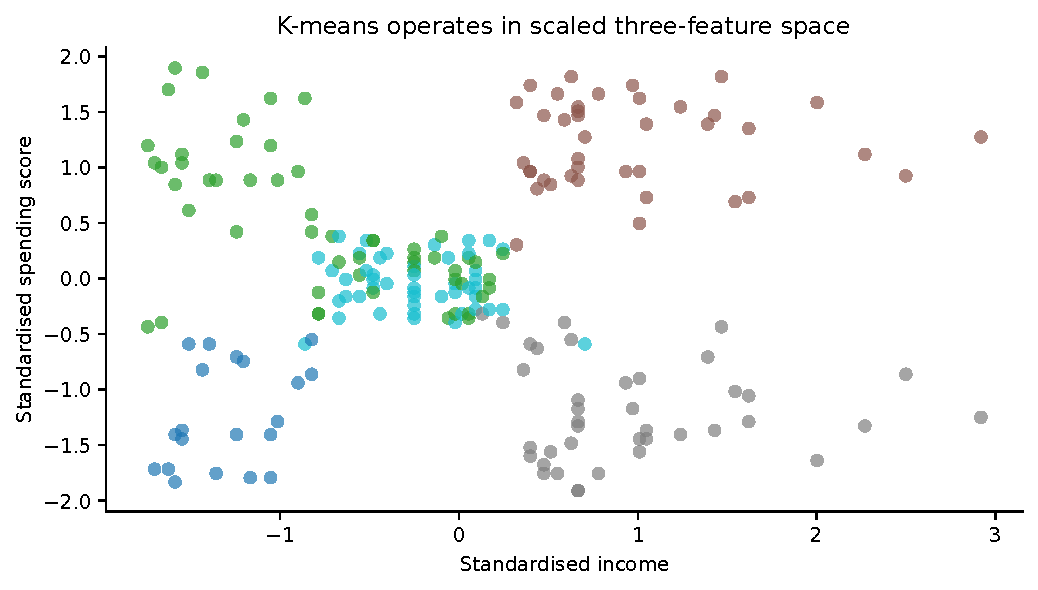
\includegraphics[width=0.76\linewidth]{figures_generated/unsupervised_kmeans_clusters.pdf}
\end{utpfig}

\section{Distance defines what ``similar'' means}
K-means uses squared Euclidean distance, so its notion of similarity is geometric and roughly spherical around cluster centres. If meaningful groups differ by density, curved shape, categorical structure, or another distance notion, k-means may be a poor representation even when it returns a numerically stable solution.

Standardisation is therefore not a routine cosmetic step: it changes the geometry on which clusters are defined.


\section{Scale before distance-based clustering}
If one feature ranges from 0 to 1000 and another from 0 to 1, Euclidean distance is dominated by the larger scale. Standardisation makes distances reflect standard-deviation units rather than raw measurement magnitude.

\begin{pitfall}
Clusters are not automatically ``real'' categories. K-means will return \(k\) clusters even when the data have no natural grouping. Interpret clusters using stability, separation, domain meaning, and external information when available.
\end{pitfall}


\section{Initialisation and stability matter}
K-means can converge to different local solutions from different starting centres. Using multiple random initialisations and comparing the best within-cluster objective reduces this instability. More importantly, analysts should check whether broad cluster assignments persist across seeds or modest perturbations of the data.

\begin{utpfig}[Elbow curve for standardised Iris measurements]{Within-cluster sum of squares must decrease as more clusters are added. The useful question is whether there is a practically meaningful bend before improvements become small.}{fig:unsup-elbow}
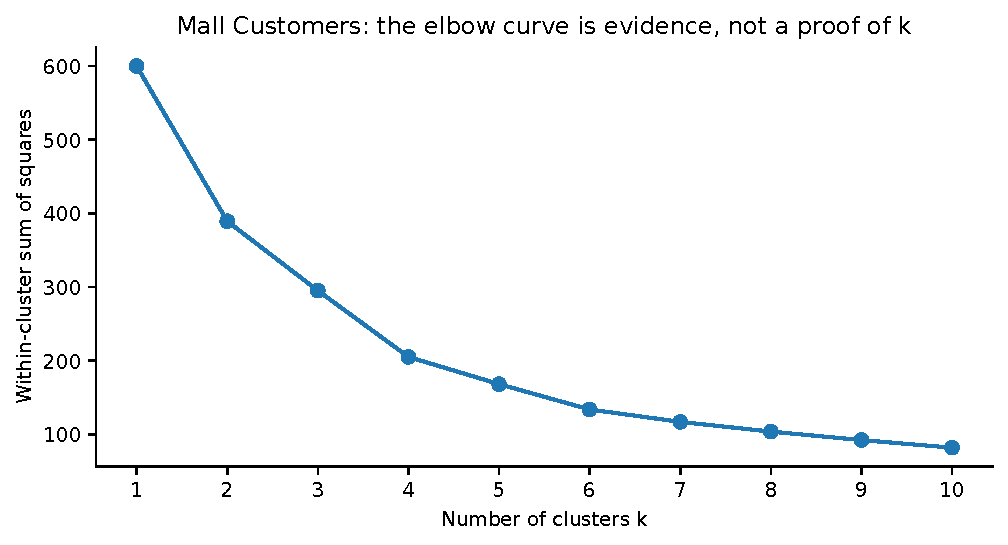
\includegraphics[width=0.78\linewidth]{figures_generated/unsupervised_elbow.pdf}
\end{utpfig}

\section{Choosing \(k\) is a modelling decision}
Use several forms of evidence: within-cluster sum of squares, silhouette-style separation, stability across random starts or resamples, and domain usefulness. No elbow plot can replace interpretation.


\section{PCA is a rotation of the numeric feature space}
After centering the features---and often scaling them when units differ---PCA finds a first direction with maximum variance. The second direction is constrained to be perpendicular to the first and captures the greatest remaining variance, and so on. Because the directions are linear combinations of the original features, PCA is most useful when correlation creates redundancy.

\begin{utpfig}[Iris observations in the first two principal components]{The first two components retain most of the variance and reveal strong separation for setosa plus overlap between the other species. Species labels are shown only for interpretation.}{fig:unsup-pca-scores}
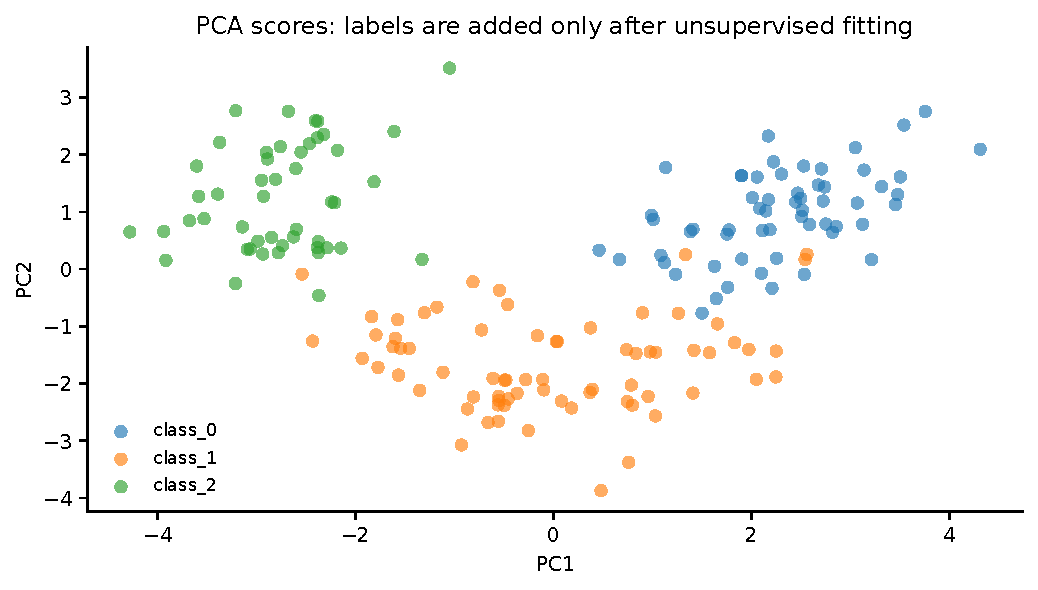
\includegraphics[width=0.76\linewidth]{figures_generated/unsupervised_pca_scores.pdf}
\end{utpfig}

\begin{utpfig}[Explained variance by component]{The bars show variance captured by each component, while the cumulative line shows how quickly information is retained as more components are kept.}{fig:unsup-pca-variance}
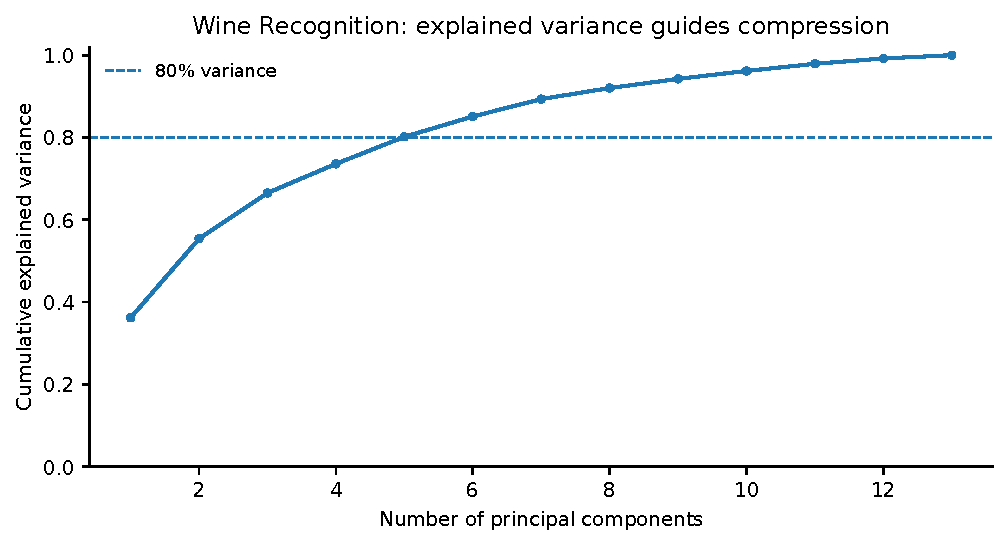
\includegraphics[width=0.78\linewidth]{figures_generated/unsupervised_explained_variance.pdf}
\end{utpfig}

\section{Principal component analysis compresses correlated features}
\term{PCA} creates orthogonal linear combinations of the original numeric variables. The first component captures the greatest possible variance; later components capture remaining orthogonal variance.

\begin{dstable}
\begin{tabularx}{\linewidth}{@{}p{3.0cm}p{4.2cm}X@{}}
\toprule
\rowcolor{DSPaleBlue!92}
PCA object & Meaning & Use \\
\midrule
Scores & coordinates of observations on components & plotting or modelling \\
Loadings & contribution of original features to components & interpretation \\
Explained variance & fraction of variability per component & decide dimensionality \\
\bottomrule
\end{tabularx}
\end{dstable}


\section{Loadings connect components back to original variables}
A principal-component score is difficult to interpret until the corresponding \term{loadings} are inspected. Large absolute loadings indicate variables that contribute strongly to that direction; signs indicate which variables move together or oppose one another along the component.

\begin{utpfig}[PCA loading directions]{Arrows show how the four standardised Iris measurements contribute to the first two principal components. Variables pointing in similar directions are positively related in this reduced space.}{fig:unsup-pca-loadings}
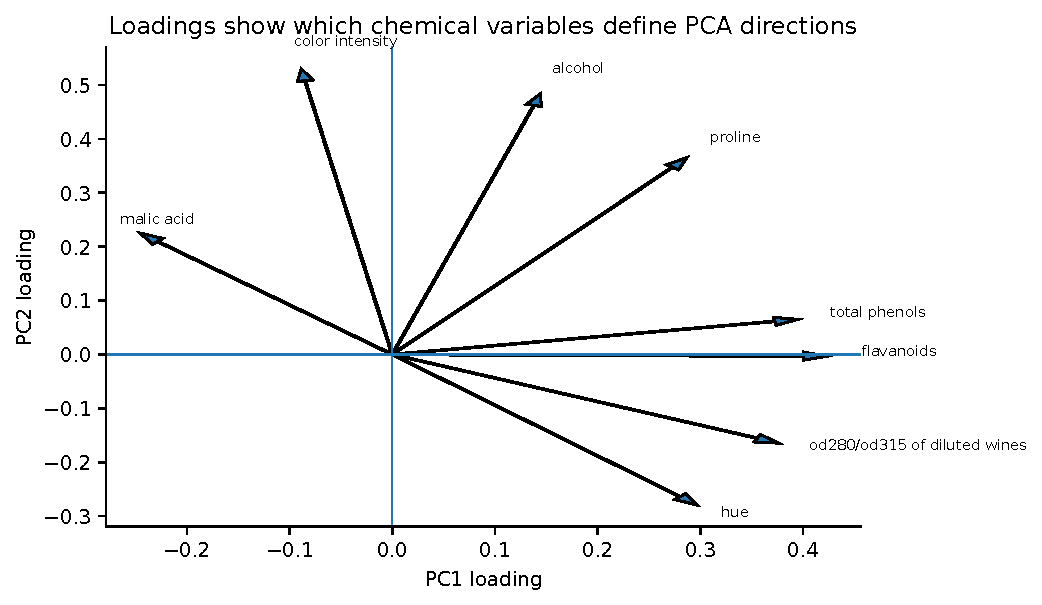
\includegraphics[width=0.70\linewidth]{figures_generated/unsupervised_pca_loadings.pdf}
\end{utpfig}

\begin{pitfall}
PCA maximises variance, not predictive usefulness or interpretability. A low-variance direction can still be important for a specific target, and a high-variance component can reflect nuisance variation. Dimensionality reduction must be evaluated against the downstream purpose.
\end{pitfall}


\section{Labels can be used after clustering for interpretation}
In the Iris lab, species labels are excluded from k-means fitting. After the clusters are created, comparing cluster assignment with species can help interpret discovered structure. This is evaluation after fitting, not supervision during fitting.

\begin{keyidea}
Unsupervised methods discover mathematical structure. Human judgment is still required to decide whether that structure is stable, meaningful, actionable, or merely an artefact of scaling and algorithm choices.
\end{keyidea}

\begin{quickcheck}
\begin{enumerate}
  \item What information is missing in unsupervised learning compared with supervised learning?
  \item Why should numeric features often be standardised before k-means?
  \item Why does requesting three clusters not prove that three natural groups exist?
  \item What is the difference between PCA scores and loadings?
\end{enumerate}
\end{quickcheck}

\section{Beyond Iris: customer segmentation and chemical profiles}

Different unsupervised methods answer different structural questions. Mall Customers asks whether observations form useful geometric segments; Wine Recognition asks whether many correlated chemical measurements can be represented in fewer dimensions.

\begin{utpfig}[Mall-customer k-means segmentation]{K-means partitions customers in income--spending space around learned centres. The five colours are algorithmic clusters, not pre-existing customer categories.}{fig:unsup-mall}
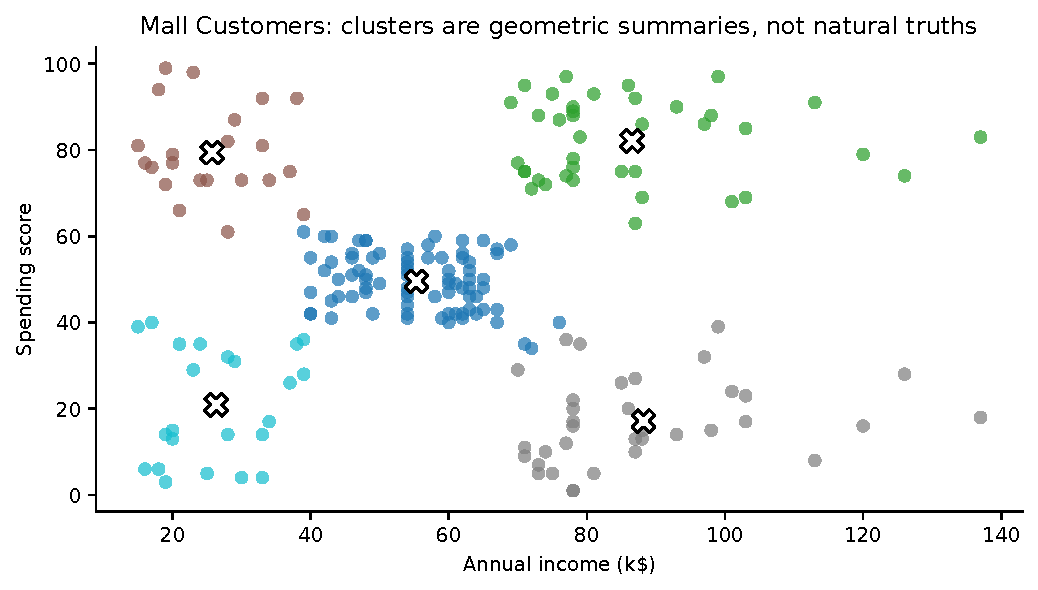
\includegraphics[width=0.78\linewidth]{figures_generated/unsupervised_mall_clusters.pdf}
\end{utpfig}

The Mall Customers file has only 200 rows, but it is pedagogically useful because cluster meaning can be inspected in original units. Adding age changes the geometry even when the displayed plot uses only income and spending score; this reminds students that a two-dimensional visualisation can omit variables used by the algorithm.

\begin{utpfig}[Wine PCA compresses 13 standardised chemical measurements]{The cultivar labels are shown only after PCA has been fitted. Separation in score space helps interpret whether the unsupervised representation captures known chemical structure.}{fig:unsup-wine}
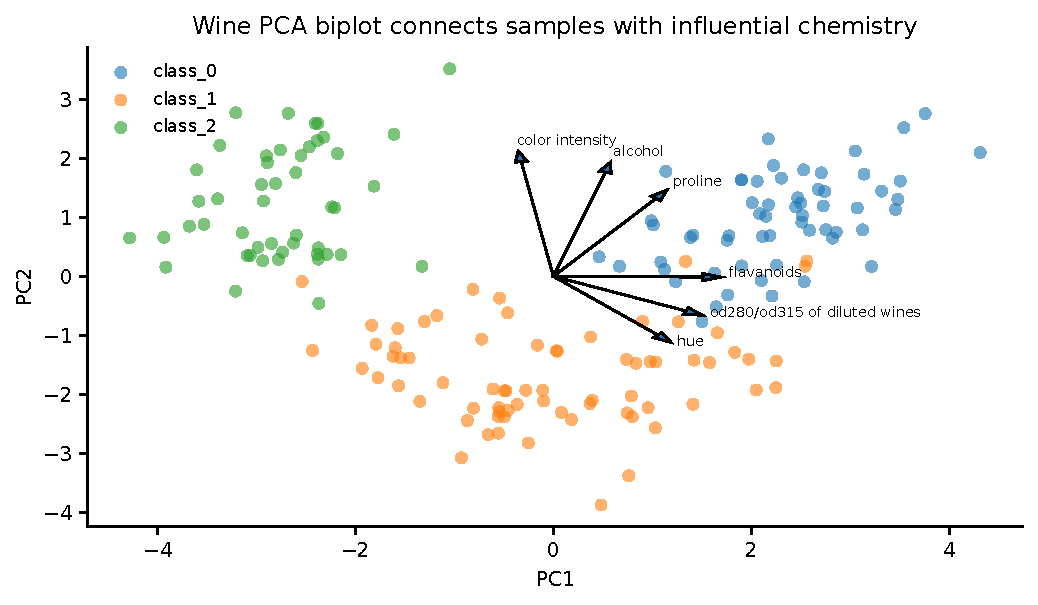
\includegraphics[width=0.80\linewidth]{figures_generated/unsupervised_wine_pca.pdf}
\end{utpfig}

PCA is particularly appropriate here because the numeric variables are measured on different scales and many describe related chemical properties. Standardisation prevents variables with large raw units, such as proline or magnesium, from dominating simply because of their measurement scale.

\begin{chapterrecap}
\begin{itemize}
  \item Unsupervised learning searches for structure without a target label.
  \item K-means is distance-based and sensitive to feature scale and initialisation.
  \item PCA represents correlated numeric features with orthogonal components.
  \item Cluster and PCA interpretations must be validated against stability and domain meaning.
\end{itemize}
\end{chapterrecap}
